% !TeX spellcheck = en_US
\documentclass[a4paper]{scrartcl}

\usepackage[utf8]{inputenc}
\usepackage[english]{babel}
\usepackage[T1]{fontenc}
\usepackage{lmodern}
\usepackage{amsmath}
\usepackage{amssymb}
\usepackage{pdflscape}
\usepackage{geometry}
\usepackage{xcolor}
\usepackage{graphicx}
\usepackage{todonotes}
\setlength{\parindent}{0pt}

\usepackage{biblatex}
\addbibresource{references.bib}


%\geometry{a4paper, top=25mm, left=30mm, right=20mm, bottom=30mm,
%headsep=10mm, footskip=12mm}

\newcommand{\itab}[1]{\hspace{0em}\rlap{#1}}
\newcommand{\tab}[1]{\hspace{.2\textwidth}\rlap{#1}}


\title{Benchmarking HDT and GraphRePair}
\author{Philip Frerk}
\date{\today}
 

\begin{document}
\maketitle

In the thesis we want evaluate the GraphRePair graph compression approach by using HDT as its benchmark. Fig.~\ref{fig:benchmark} shows the general aspects of a compression process applied to a RDF graph. $p_{input}$ and $p_{alg}$ are benchmark parameters, this means they can be changed during the evaluation. In contrast, $m_{output}$ and $m_{runtime}$ are measures which we want to evaluate.

\begin{figure}[h]
	\centering
	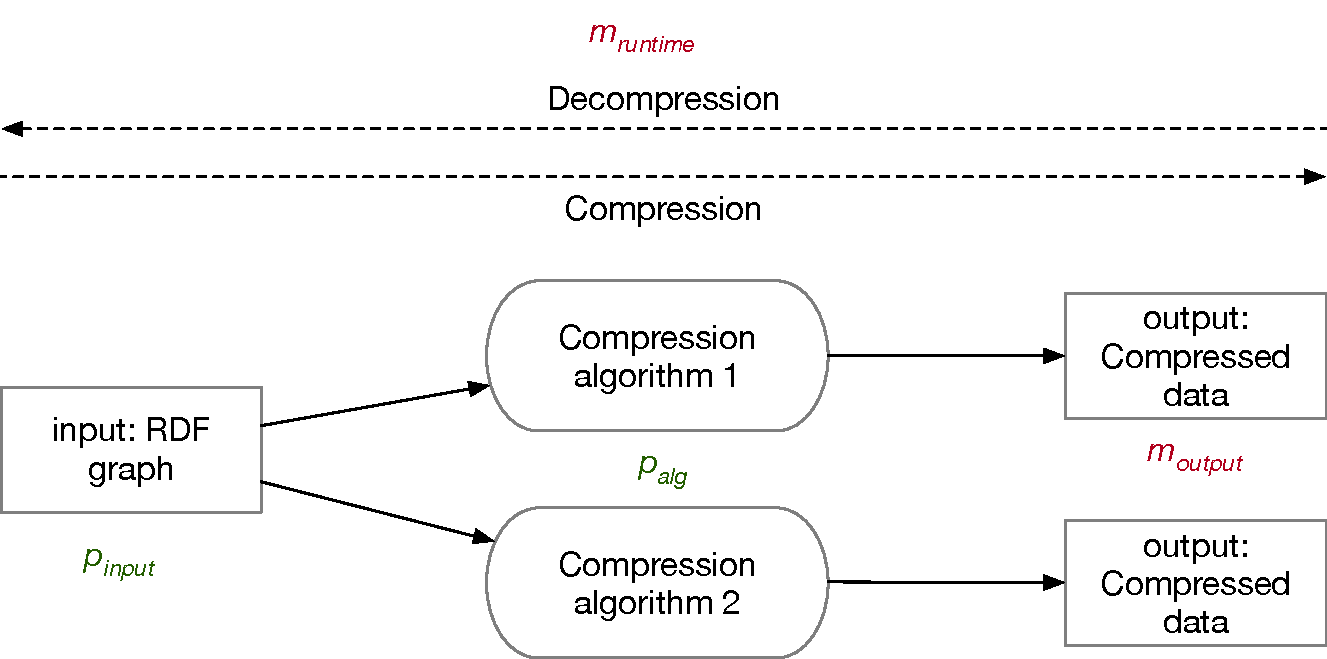
\includegraphics[width=1\textwidth]{Benchmark_fig}
	\caption{The different aspects of a compression process. $p_{input},p_{alg}$ are parameters that can be changed. $m_{output},m_{runtime}$ are measures of the algorithm's performance.}
	\label{fig:benchmark}
\end{figure}

We want to analyze the influence of different values for the parameters on the output measures. The following list explains the parameters and measures.


\begin{itemize}
	\item $ (p_{input}) $ RDF graph: Parameters of the input data
		\begin{itemize}
			\item format (ttl, xml, ...)
			\item \#edges, \#nodes, average node degree,...
			\item percentage of literals
			\item percentage of blank nodes
			\item 'HDT pattern similarity' (star pattern):one or several node(s) that appear in many triples as subject(s)\\
						(HDT benefits from this pattern)
			\item 'GraphRePair pattern similarity': More difficult, many occurrences of one or several digrams appear\\
			(GraphRePair benefits from this pattern)
		\end{itemize}
	\item \textbf{$ (p_{alg}) $} Compression algorithm: Parameters of the algorithms
	\begin{itemize}
		\item hardware environment
		\item multi threading / single threading
	\end{itemize}
	\item \textbf{$ (m_{output}) $} Compressed data:\\
	The size of the compressed data (similarly the compression ratio) is the core measurement of a compression algorithm.
	\begin{itemize}
		\item size of output file compared the size of the original file
	\end{itemize}
	\item \textbf{$ (m_{runtime}) $} (De)-Compression\\
	Obviously the run time of the compression is very important. Additionally, the decompression is interesting, because sometimes the user wants to decompress the data since some operations might not be possible to do with the compressed data.
	\begin{itemize}
		\item run time
	\end{itemize}
\end{itemize}

\section*{Generating Artificial RDF Data}

For the evaluation of compression algorithms, real data is often used to show that the algorithms work well in reality. In a direct comparison of two algorithms (benchmark), real data is not well suited, because here we want to investigate which algorithm works better for which parameter values. Therefore, it is necessary to generate artificial data that precisely fulfill these parameter values. A big task of the thesis will be the generation of such data.

\subsection*{Generating a single RDF Graph}

We will now discuss the generation of some different input parameters ($ p_{input} $). 

\begin{itemize}
	\item format: trivial
	\item \# edges / \# nodes: trivial
	\item average node degree: for each node generate random number of incident edges: standard deviation of random number has to be defined
	\item percentage of literals: Let $n$ be the number of nodes. Then we are evaluating $\frac{l}{n} \in [0,1]$ where $l$ is the absolute number of literals. So we have to fix $n$ first and then $l$
	\item percentage of blank nodes: Let $n$ be the number of nodes. Then we are evaluating $ \frac{b}{n} \in [0,1]$ where $b$ is the absolute number of blank nodes. So we have to fix $n$ first and then $b$
	\item 'HDT pattern similarity': Determine number of 'frequent subject nodes' (FSN). Then determine average number of triples a single FSN appears in (as subject)
	\item 'GraphRePair pattern similarity': Determine class of digram (many different such classes exist). Then determine number of occurrences.
	
	The goal is to define a property $p_{GPR} \in [0,1]$ for an RDF graph, such that the higher  $p_{GPR}$ is, the higher the graph can theoretically be compressed by GraphRePair.  $p_{GPR}$ should be defined in such a way that we can generate a partially random RDF graph with a pre-determined value for  $p_{GPR}$. We can then construct a plot with  $p_{GPR}$ on the horizontal axis and the compression ratio on the vertical axis (for different graphs with different values for $p_{GPR}$) and analyze if our hypothesis about the impact of  $p_{GPR}$ is correct.

A possible way of defining  $p_{GPR}$ is the following:

\[
 p_{GPR}= \dfrac{\sum_{d \in \text{digrams with } |occ(d)|>1} (|occ(d)|) }{n} \in [0,1]
\]

Here we count the sum of all occurrences of digrams with more than one occurrence and finally divide the sum by $n$ which is the number of nodes of the graph. $occ(d)$ is defined as the set of all occurrences of the digram $d$.

We only count occurrences of digrams with more than one occurrence because only digrams with multiple occurrences can have a positive impact on the compression ratio (in most cases).

A further intention of the definition of $p_{GPR}$ is that this property should not influence the compression ratio of HDT. That could be achieved by choosing digram types that HDT does not benefit from. It must be investigated what those types are.

In order to make the definition of $p_{GPR}$ clearer, we will look at an example from the GraphRePair paper.

\begin{figure}[h]
	\centering
	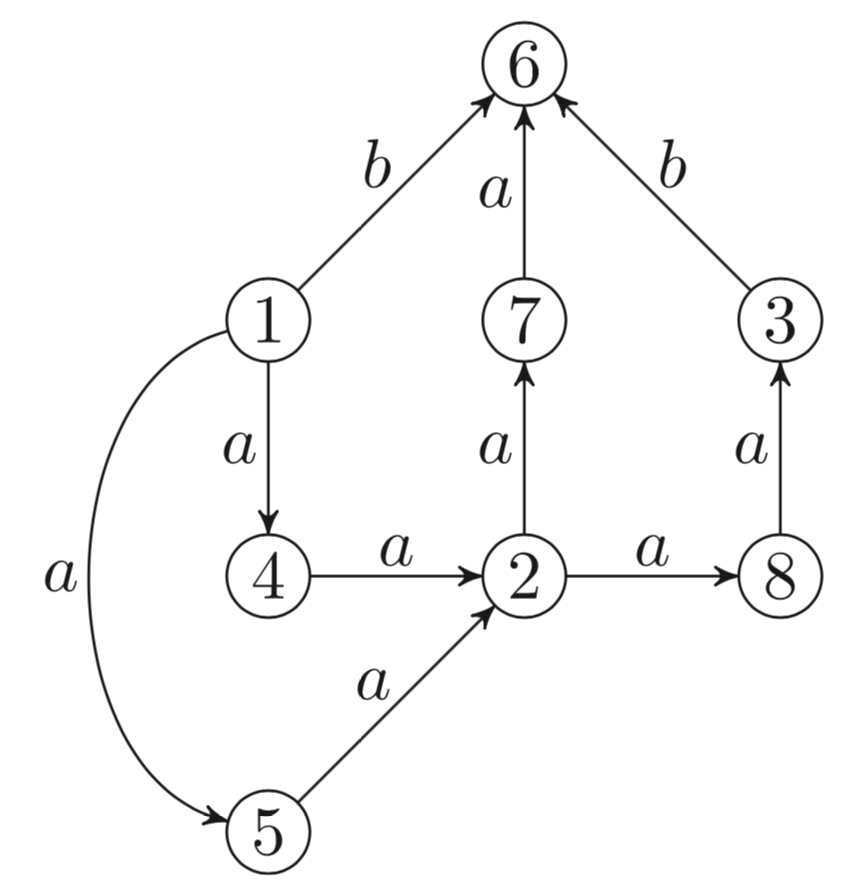
\includegraphics[width=0.3\textwidth]{img/uncompressed}
	\caption{An uncompressed graph.}
	\label{fig:uncompressed}
\end{figure}

\begin{figure}[h]
	\centering
	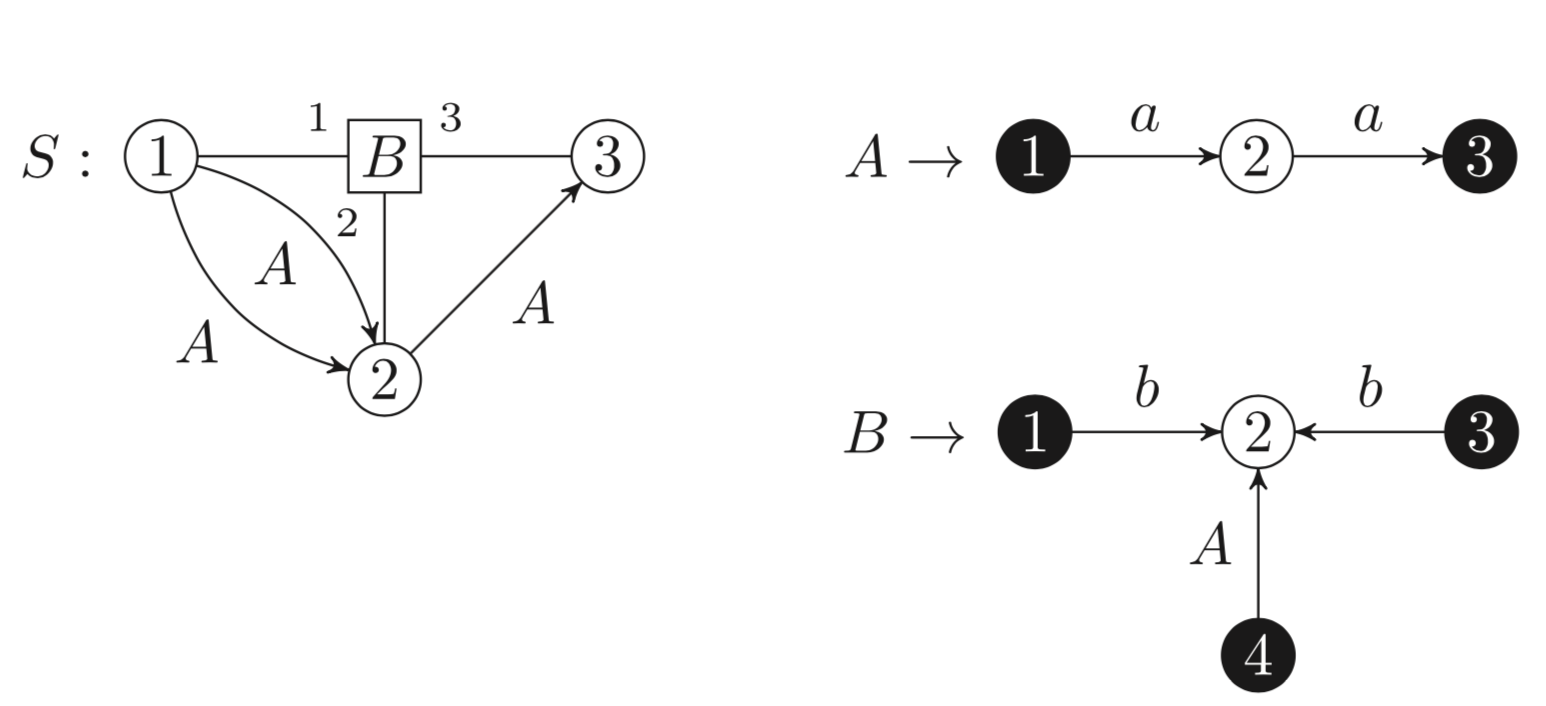
\includegraphics[width=0.6\textwidth]{img/compressed}
	\caption{The compressed graph from Fig.~\ref{fig:uncompressed} with the digrams A and B.}
	\label{fig:compressed}
\end{figure}

In Fig.~\ref{fig:uncompressed} you see an uncompressed graph with 8 nodes. In Fig.~\ref{fig:compressed} you see the compressed version of the graph and its two digrams A and B. A is a 'simple' digram as it contains no other digrams, but B contains one occurrence of A. Therefore we have to count one occurrence of A for each occurrence of B. The value of $p_{GPR}$ is the following in this case:

\[
p_{GPR}= \dfrac{\sum_{d \in \text{digrams with } |occ(d)|>1} (|occ(d)|) }{n} = \dfrac{|occ(A)|}{8} = \dfrac{4}{8}
\]

According to the definition of $p_{GPR}$ the one occurrence of B is not considered (but the one occurrence of A in B is counted).
\\\\
There are now two directions of handling the property $p_{GPR}$:

\begin{enumerate}
	\item Generate a new graph with a pre-defined value for $p_{GPR}$
	\item Compute the value for $p_{GPR}$ of a given graph
\end{enumerate}

The first direction seems to be the easier one. We can define a set of digrams for which we want to generate multiple occurrences. Then we generate a graph triple by triple. For some triples we just use random values, for others we insert occurrences of one of the defined digrams. Furthermore we want to make sure that the different occurrences do not overlap, as this would decrease the potential compression ratio. Due to the randomness it will happen that we do not precisely achieve the pre-defined $p_{GPR}$-value, but an approximation should work.

The second direction is completely different. It could be interesting to analyze the $p_{GPR}$-value for a given graph, e.g. from DBPedia. But this is more difficult, because in order to count the occurrences of the different digrams we would have to act like the GraphRePair algorithm. One possibility would be to use the algorithm as a white box and note what different  digram occurrences it finds.

\end{itemize}


\subsection*{Generating multiple RDF Graphs}

The general idea  of the benchmark is that there are certain parameters HDT benefits from (e.g. 'HDT pattern') and others from which GraphRePair benefits (e.g. 'GraphRePair pattern').

The end product should take an RDF graph as input and predict whether it will be better compressed by HDT or GraphRePair. To achieve that we have to compare different parameters directly and compute thresholds for them indicating that above this threshold one of the algorithms works better.

It would also be possible to ask the user whether he rather wants an acceptable runtime and moderate compression rate or a good compression ratio at longer runtime. However, it is likely that HDT in general will have a better runtime as it has been implemented more professionally.

In order to achieve this we must generate RDF graphs that partially fulfills one of the HDT beneficial patterns and at the same time partially fulfills some of the GraphRePair beneficial patterns. Then we can evaluate the measures (compr. ratio and run time) on these graphs and determine the thresholds mentioned above.


\section*{New Insights  from Maneth Paper}

\begin{itemize}
	\item Storage of dictionary is omitted => we need algorithm for dictionary compression and add the storage to the overall storage
	\item Node order has marginal input on compr. ratio for RDF
	\item Comparison only with $k^2$-tree compressor
	\item No. of equivalence classes has correlation with compression ratio (two nodes have a similar equiv. class if their neighborhood is similar => repeating sub-structures). Therefore: The lower the number, the better the compr. ratio.
	\item star pattern has also correlation with compr. ratio 
	\item Graphs that are also tree-like compress well, because in every iteration halves the number of edges around the hub node (Why???)
\end{itemize}


\section{Evaluation Results}

The evaluation scenario is the following:

All graphs have the same amount of triples (1199) and nodes (1200). The first graph has only one subject (all other nodes are objects). The next one has 40+1 subjects and so on. In each graph the amount of subjects is 40 more than in the previous graph.

The following results show the compression ratios ($ \frac{\text{compr. size}}{\text{orignal size}} $) for the compressors HDT and GraphRePair (GRP) for the scenario described above.


Here is an overview of what the different results show:

\begin{itemize}
  \item Fig.~\ref{fig:bothWithDict}: Both, 1 predicate, dictionary size included
  \item Fig.~\ref{fig:bothWithDict1000Predicates}: Both, 1000 predicates, dictionary size included
  \item Fig.~\ref{fig:hdtWithoutDict}: HDT, 1 predicate, dictionary size not included
  \item Fig.~\ref{fig:grpWithoutDict}: GRP, 1 predicate, dictionary size not included
\end{itemize}

%\begin{figure}[h]
%	\centering
%	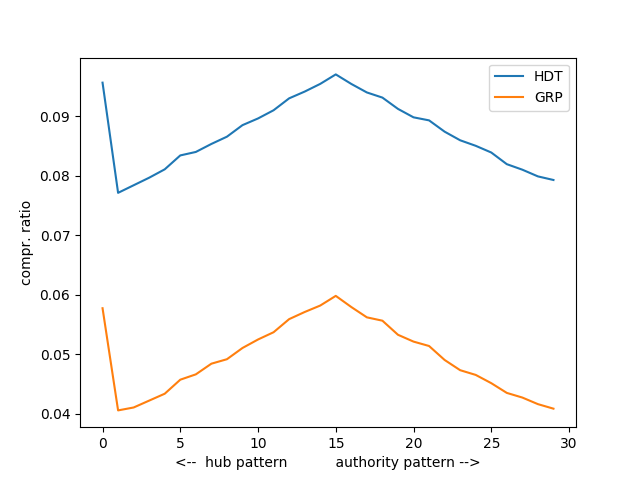
\includegraphics[width=\textwidth]{img/eval/bothWithDict}
%	\caption{Compression ratio (dictionary size included) for the series of graphs. Graphs have only one distinct predicate.}
%	\label{fig:bothWithDict}
%\end{figure}
%
%
%\begin{figure}[h]
%	\centering
%	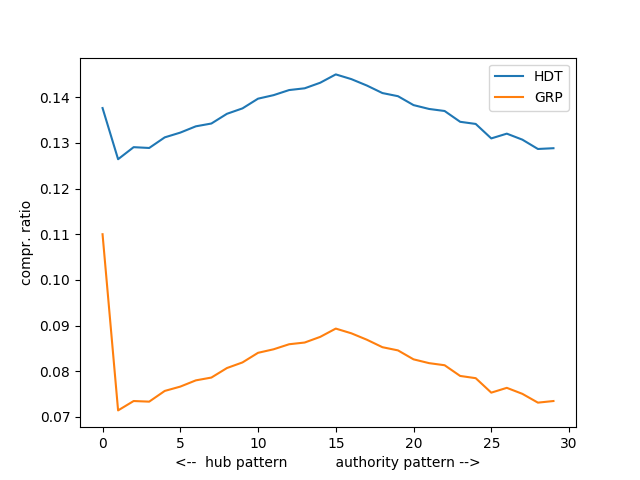
\includegraphics[width=\textwidth]{img/eval/bothWithDict1000Predicates}
%	\caption{Compression ratio (dictionary size included)  for the series of graphs. Graphs have 1000 distinct predicates.}
%	\label{fig:bothWithDict1000Predicates}
%\end{figure}
%
%\begin{figure}[h]
%	\centering
%	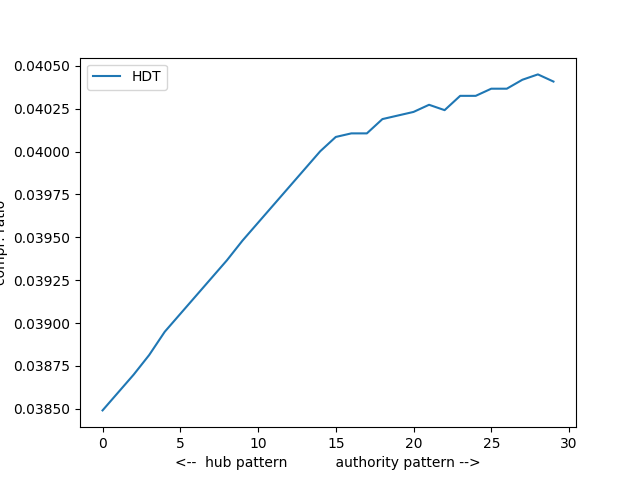
\includegraphics[width=\textwidth]{img/eval/hdtWithoutDict}
%	\caption{HDT Compression ratio (dictionary size not included)  for the series of graphs. Graphs have only one predicate.}
%	\label{fig:hdtWithoutDict}
%\end{figure}
%
%\begin{figure}[h]
%	\centering
%	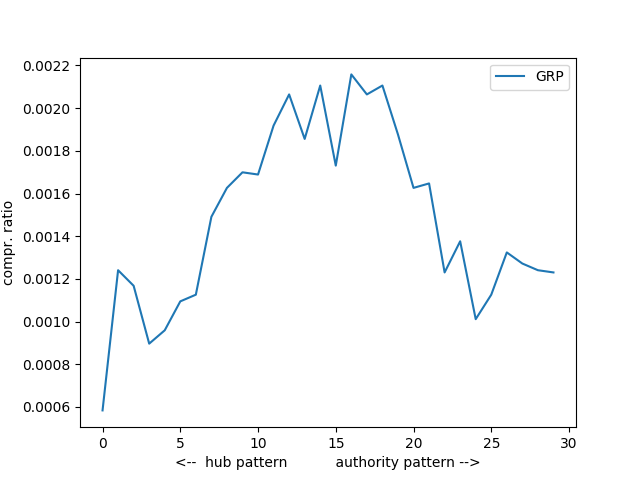
\includegraphics[width=\textwidth]{img/eval/grpWithoutDict}
%	\caption{GRP Compression ratio (dictionary size not included)  for the series of graphs. Graphs have only one predicate.}
%	\label{fig:grpWithoutDict}
%\end{figure}

\section{Ideas for further work}


\begin{itemize}
	\item (De)-Compr. time evaluation for HDT and GRP (quite trivial, because HDT is way faster, but it is necessary to mention this)
	\item Improvement of GRP in terms of RDF
	\begin{itemize}
		\item using symmetric predicates => Are there many? How difficult to implement?
		\item Further ideas needed: (e.g. node visiting order has only small effect with RDF)
		\item Problem: Code not documented, therefore difficult to extend it.
	\end{itemize}
	\item Deeper analysis of GRP
	\begin{itemize}
		\item Where does the low compr. ratio come from? (grammar or $ k^2 $)
		\item Which features/properties of an RDF graph lead to low/high grammar/$ k^2 $ compr. ratio? => E.g. divide compr. ratio in grammar ratio and $k^2$ ratio, investigate which ratio makes which part of the total ratio
		\item Investigate, which kind of digrams are often found in RDF. E.g. star pattern seems well suited for GRP, why is that the case? Which digram does it find here?
	\end{itemize}
	\item Comparison to a node-based grammar compressor:
	\begin{itemize}
			\item GRP is an edge-based compressor as it replaces edges. In contrast, Dürksen's algorithm is node-based. It could be investigated which one leads to a higher compr. ratio.
			\item \enquote{For future work, there are several paths to follow. It would be interesting to consider a RePair compression scheme for graphs that is based on node replacement (NR) graph grammars (see e.g. [48]). NR graph grammars can compress some graphs, e.g. cliques, much stronger than HR grammars. On the other hand, rules of NR grammars are more complex due to the additional con- nection relation and thus more expensive to store.} [Maneth]
	\end{itemize}
\end{itemize}

\section{OWL}

Interesting OWL Constructs
\begin{itemize}
	\item SymmetricProperty (evtl alles materialsieren), TransitiveProperty (wahrscheinlich alles ent-materialisieren)
	\item equivalentProperty: Establish mapping from prop to List<Prop>, in all triples where some p in List<Prop> occurs, replace it with prop => more repeating predicates!
\end{itemize}

\section{Results Materialisation}
 File: mappingbased-properties\_en.ttl (first 500k triples)
 
 
\begin{figure}
	\centering
	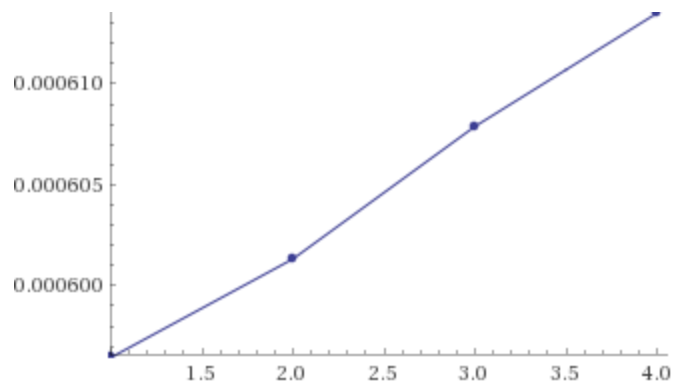
\includegraphics[width=0.7\linewidth]{img/evalMat/ratios}
	\caption{Compr. ratios: Original, inverse, symmetric, transitive}
	\label{fig:ratios}
\end{figure}

\begin{figure}
	\centering
	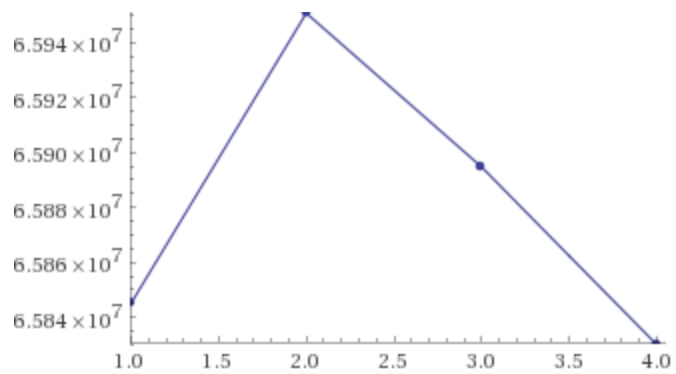
\includegraphics[width=0.7\linewidth]{img/evalMat/sizes}
	\caption{Original file sizes: Original, inverse, symmetric, transitive}
	\label{fig:sizes}
\end{figure}

Symmetric: http://dbpedia.org/ontology/spouse
\\\\
Transitive:

0 = "http://dbpedia.org/ontology/isPartOf"

1 = "http://dbpedia.org/ontology/province"

2 = "http://dbpedia.org/ontology/locatedInArea"

3 = "http://dbpedia.org/ontology/city"

4 = "http://dbpedia.org/ontology/district"

5 = "http://dbpedia.org/ontology/county"

6 = "http://dbpedia.org/ontology/settlement"
\\\\
Inverse:

"http://dbpedia.org/ontology/doctoralStudent" -> "http://dbpedia.org/ontology/doctoralAdvisor"

"http://dbpedia.org/ontology/mother" -> "http://dbpedia.org/ontology/child"

"http://dbpedia.org/ontology/father" -> "http://dbpedia.org/ontology/child"

 "http://dbpedia.org/ontology/child" -> "http://dbpedia.org/ontology/mother"
 
 "http://dbpedia.org/ontology/follows" -> "http://dbpedia.org/ontology/followedBy"
 
 "http://dbpedia.org/ontology/followedBy" -> "http://dbpedia.org/ontology/follows"
 
 "http://dbpedia.org/ontology/doctoralAdvisor" -> "http://dbpedia.org/ontology/doctoralStudent"
 
 "http://dbpedia.org/ontology/spouse" -> "http://dbpedia.org/ontology/spouse"



\section{Fragen an Michael}

\begin{itemize}
	\item Materialiserung scheint nicht viel zu bringen. Nur ein symmetrisches Prädikat?? \\
	Andere Möglichkeit: Alles entmaterialisieren und dann zeigen dass man weniger speichern muss, auch wenn man die Ontologie abspeichert. 
	\item Blank nodes: Konvertierung von string nach int wahrscheinlich nicht nötig, da in der Impl von dem dict sowieso nur Zahlen gespeichert werden.\\
	Speichern von Blank node IDs evtl gar nicht nötig??
	\item Literale: Kompr. mit Huffman; einen Huffman Code für alle Literale
\end{itemize}

















\end{document}